%%% Local Variables: 
%%% mode: latex
%%% TeX-master: "../main"
%%% End: 

%\chapter{外文资料的原文}
%\label{cha:engorg}
%
%\section{Abstract}
%
%Research efforts on 3DTV technology have been strengthened worldwide recently, covering the whole media processing chain from capture to display. Different 3DTV systems rely on different 3-D scene representations that integrate various types of data. Efficient coding of these data is crucial for the success of 3DTV. Compression of pixel-type data including stereo video, multiview video, and associated depth or disparity maps extends available principles of classical video coding. Powerful algorithms and open international standards for multiview video coding and coding of video plus depth data are available and under development, which will provide the basis for introduction of various 3DTV systems and services in the near future. Compression of 3-D mesh models has also reached a high level of maturity. For static geometry, a variety of powerful algorithms are available to efficiently compress vertices and connectivity. Compression of dynamic 3-D geometry is currently a more active field of research. Temporal prediction is an important mechanism to remove redundancy from animated 3-D mesh sequences. Error resilience is important for transmission of data over error prone channels, and multiple description coding (MDC) is a suitable way to protect data. MDC of still images and 2-D video has already been widely studied, whereas multiview video and 3-D meshes have been addressed only recently. Intellectual property protection of 3-D data by watermarking is a pioneering research area as well. The 3-D watermarking methods in the literature are classified into three groups, considering the dimensions of the main components of scene representations and the resulting components after applying the algorithm. In general, 3DTV coding technology is maturating. Systems and services may enter the market in the near future. However, the research area is relatively young compared to coding of other types of media. Therefore, there is still a lot of room for improvement and new development of algorithms.
%
%\section{Introduction}
%
%Extending visual sensation to the third dimension has been investigated over decades. However, significant consumer mass markets haven't developed yet. 3-D video is established in niche markets, including professional applications (e.g., scientific visualization, medicine) and entertainment (IMAX cinemas, 3-D gaming). In recent years, research efforts have been strengthened worldwide to remove technological obstacles that encumber wider success of 3-D video applications \onlinecite{smolic20063d, onural2004overview, smolic20043dav, smolic2005interactive, onural2006assessment}. Significant improvements have been achieved for all components of the processing chain, from acquisition and signal processing, over 3-D scene representation, coding and transmission, to rendering and 3-D display. Very likely various 3-D video systems, components, applications and services will enter the market in the near future.
%
%Overviews of the state-of-the-art of technology for 3-D video are given in different papers of this Special Issue, each focusing on a specific component of the processing chain. This paper is devoted to coding. Various 3-D scene representation formats are used in different 3-D video systems and applications as de- scribed in \onlinecite{alatan2007scene}. These formats integrate various types of data, such as multiview video, and geometry data in form of depth or 3-D meshes. In general, 3-D video results in a tremendous amount of data that needs to be transmitted, stored or watermarked. Therefore, efficient compression is a key condition for the success of 3-D video. There is also a strong necessity for developing robust 3-D watermarking techniques, which protect the ownership rights. Further, the availability of open international standards is in general an important enabling factor for the development of markets in the media business. ISO/IEC JTC1/SC29/WG11 (Moving Picture Experts Group—MPEG) is one of the international standardization bodies that play an important role in digital media standardization. Therefore, this paper highlights MPEG standards for the different data as available and under development.
%
%The following section gives an overview of coding of multiview video, depth and associated data, with focus on avail- able and emerging MPEG standards. Section III is devoted to compression of static and dynamic 3-D mesh data as used for 3-D video representations as well as for 3-D computer graphics. Error resilience and multiple description coding (MDC) for 3-D is outlined in Section IV. Then, Section V elaborates on protection of 3-D content using watermarking. Finally, Section VI summarizes and concludes the paper.
%
%\section{Coding of Multiview Video, Depth, and Associated Data}
%
%Many 3DTV systems are based on scenarios, where a 3-D scene is captured by a number of cameras (see e.g., \onlinecite{tanimoto2004free, fujii2002free, matsuyama2004real, hamaguchi2003real, carranza2003free, wurmlin20033d, wurmlin20043d, matusik20043d}). The simplest case is classical stereo video with two videos. More advanced systems apply 8, 16, and more cameras. Some systems additionally apply per sample depth data that can also be treated as video signals. This section gives an overview of compression algorithms and standards for such data. An early overview of this research area can be found in \onlinecite{shum2003survey}. Depending on the degree of common content, shared by a subset of the cameras, a coding gain can be achieved in comparison to single-view coding. In multiview coding, correlations between adjacent cameras are exploited in addition to temporal correlations within each sequence. Therefore, multiview coding adds an- other compression dimension on top of single-view coding: the inter-view direction.
%
%\subsection{Conventional Stereo Video Coding}
%Stereo view is the most important special case of multiview with views. Compression of conventional stereo video has been studied for a long time and the corresponding standards are available. A conventional stereo pair consists of two images showing the same scene from two slightly different viewpoints corresponding to the distance of human eyes. The images are in general very similar, which makes them well suited for compression, e.g., with one image predicting the other. For instance one of them can be compressed without reference to the other stereo image. Then, the second image can be predicted from the already encoded one, just like temporally related images can be motion-compensated in video compression.
%
%The samples of both images correspond to each other through the 3-D geometry of the scene and camera properties, including positions and internal camera parameters such as the focal length. The displacement or disparity of each sample in one image with respect to the other is equivalent to a dense motion field in between two consecutive images of a video sequence. Therefore, it is justified to use the same principles of motion estimation and motion compensation for disparity estimation and disparity compensation for image prediction and then to only encode the prediction error or residual further.
%
%Nevertheless, some specific differences between motion compensation and disparity compensation need to be considered. The statistics of disparity vector fields is different from the statistics of motion vector fields. Disparities are biased and relatively large. Zero disparity means a very large depth of the corresponding point in 3D, while 3-D points close to the camera may have very large disparity values. This may require adjustments of entropy coding of the disparity vectors. In general temporally adjacent images of a video sequence tend to be more similar than views of a stereo pair at practical frame rates. Disocclusion effects, i.e., content that is visible in one image is occluded in the other and can therefore not be predicted, are on average more evident in a stereo pair than in between two temporally adjacent video images. Further, specific differences in a stereo pair may come from incorrect white and colour balance but also due to scene lighting and surface reflectance effects.
%
%\begin{figure}[htbp]
%\begin{center}
%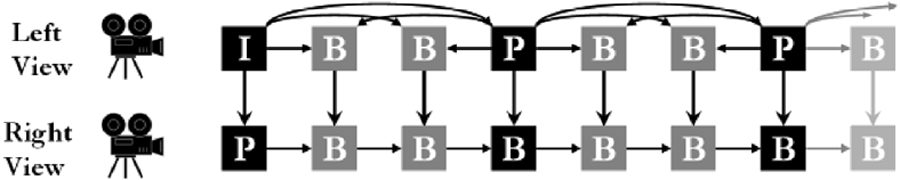
\includegraphics[width=0.8\textwidth]{predh262.png}
%\caption{Illustration of prediction in H.262/MPEG-2 Video multiview profile}
%\label{fig:predh262}
%\end{center}
%\end{figure}
%
%
%The combination of inter-view and temporal prediction is the basic principle for efficient compression of conventional stereo video. A corresponding standard specification has already been defined in ITU-T Rec. H.262/ISO/IEC 13818-2 MPEG-2 Video, the Multiview Profile \onlinecite{haskell1997digital, itu1994mpeg2}, as illustrated in Fig. \ref{fig:predh262}. The left eye view is encoded without reference to the right eye view, using standard MPEG-2. This ensures backward compatibility with Main Profile of H.262/MPEG-2 Video, since it is possible to decode the left eye view bit stream and to display 2-D video. For the right eye view, inter-view prediction is allowed in addition to temporal prediction.
%
%However, the gain in compression efficiency compared to independent encoding of both video streams is rather limited. This is mainly due to the fact that temporal prediction already provides very good performance. Typically, if temporal prediction is efficient for a certain image (e.g., B-pictures for right view in Fig. \ref{fig:predh262}) then additional inter-view prediction does not increase the coding performance significantly. Temporal neighbouring images are typically on average more similar than spatially neighbouring images.
%
%For images that are coded as I-pictures, i.e., without reference to other temporally adjacent images in the video sequence, a significant gain can be achieved by inter-view prediction. Typically every 0.5–1 s such I-pictures are inserted into a video stream to enable random access and error robustness. In Fig. \ref{fig:predh262}, the left-hand side picture of the left view is encoded as I-picture. The corresponding left-hand side picture of the right view would also be encoded as I-picture for random access when in- dependently encoding both video streams. However, in H.262/ MPEG-2 Video multiview coding, inter-view prediction can be applied, resulting in a significant increase of compression efficiency compared to coding this picture as I-picture.
%
%Research on compression of conventional stereo video has continued into several directions, including for instance optimum joined bit allocation for both channels, or abandoning backward compatibility to design more efficient inter-view prediction structures. Algorithms have been based on more up-to-date video codecs such as H.263\onlinecite{itu1995h263}, MPEG-4 Visual\onlinecite{itu1999mpeg4}, or H.264/AVC\onlinecite{sun2005stereo, wiegand2003overview, itu2003h264}. However, none of the developments including the original Multiview profile have reached commercial relevance so far, since the application of stereo video did not develop into a relevant mass market yet.
%
%\subsection{Compression of Video Plus Depth Data}
%
%An alternative to classical stereo video as described in the previous section is to transmit a video signal and a per sample depth map. From the video and depth information, a stereo pair can be rendered at the decoder \onlinecite{fehn2002evolutionary, fehn20043d}. This extends the functionality since it enables head motion parallax viewing if the user’s head motion is tracked. Additionally, this format is interesting from compression efficiency point of view. Per sample depth data can be regarded as a monochromatic, luminance-only video signal. The depth is restricted to a range between two extremes $Z_{near}$ and $Z_{far}$ indicating the minimum and maximum distance of the corresponding 3-D point from the camera respectively. The depth range is linearly quantized with 8 bit, i.e., the closest point is associated with the value 255 and the most distant point is associated with the value 0. With that, the depth map is specified, resulting in a grey scale image. These grey scale images can be fed into the luminance channel of a video signal and the chrominance can be set to a constant value. The resulting standard video signal can then be processed by any state-of-the-art video codec.
%
%Results from the European ATTEST project \onlinecite{fehn2002evolutionary} have shown that depth data can be very efficiently compressed this way. Several state-of-the-art video codecs have been tested (MPEG-2, MPEG-4, H.264/AVC). A course estimate indicates that 10\%–20\% of the bit rate which is necessary to encode the colour video is sufficient to encode the depth at good quality. This is due to the specific statistics of depth data, being on average smoother and less structured that colour data.
%
%Based on these observations, a new backward compatible (with respect to classical DVB) approach for 3DTV was developed in the ATTEST project. It uses a layered bit stream syntax. The base layer is a conventional 2-D colour video encoded using MPEG-2. This base layer can be processed by any existing MPEG-2 decoder providing backward compatibility. Additionally the bit stream contains an advanced layer carrying the encoded depth information. Advanced systems may access this layer to decode the depth stream and then generate a stereo pair to be displayed stereoscopically by view interpolation.
%
%This concept is highly interesting due to the backward compatibility, compression efficiency and extended functionality compared to conventional stereo video. Moreover, it does not introduce any specific coding algorithms. It is only necessary to specify high-level syntax that allows a decoder to interpret 2 incoming video streams correctly as colour and depth. Additionally information about depth range($Z_{near}$ and $Z_{far}$) needs to be transmitted. Therefore, MPEG specified a corresponding container format “ISO/IEC 23002-3 Representation of Auxiliary Video and Supplemental Information,” also known as MPEG-3 Part 3, for video plus depth data \onlinecite{iso2007rep, iso2007fdam}. Moreover, H.264/AVC contains an option to convey the depth images through its auxiliary picture syntax. Here, the video codec for the colour video signal and associated depth video signal are both H.264/AVC. This approach is backwards compatible with any existing deployment of H.264/AVC.
%
%A general problem of the video plus depth format is content creation, i.e., the generation of depth information. Cameras that automatically capture per pixel depth with the video are available and are being further enhanced, but the quality of the captured depth fields is currently still limited. Algorithms for depth estimation have been studied extensively in computer vision literature and powerful solutions are available. However, it always remains an estimation that can only be solved up to a residual error probability. Estimation errors influence the quality of rendered views. A fully automatic, accurate and reliable depth capturing system is still to be developed. User-assisted content generation is an option for specific applications. Even having perfect depth available, artifacts may occur in rendered views due to disocclusion. This effect increases with the distance of the virtual view from the original camera position. Additional occlusion layers (layered depth video as extension of layered depth images \onlinecite{shade1998layered}) or extension to multiview video plus depth \onlinecite{zitnick2004high, kauff2007depth}, help to minimize these problems at the cost of increased data rate and complexity.
%
%\subsection{Multiview Video Coding}
%
%\begin{figure}[htbp]
%\begin{center}
%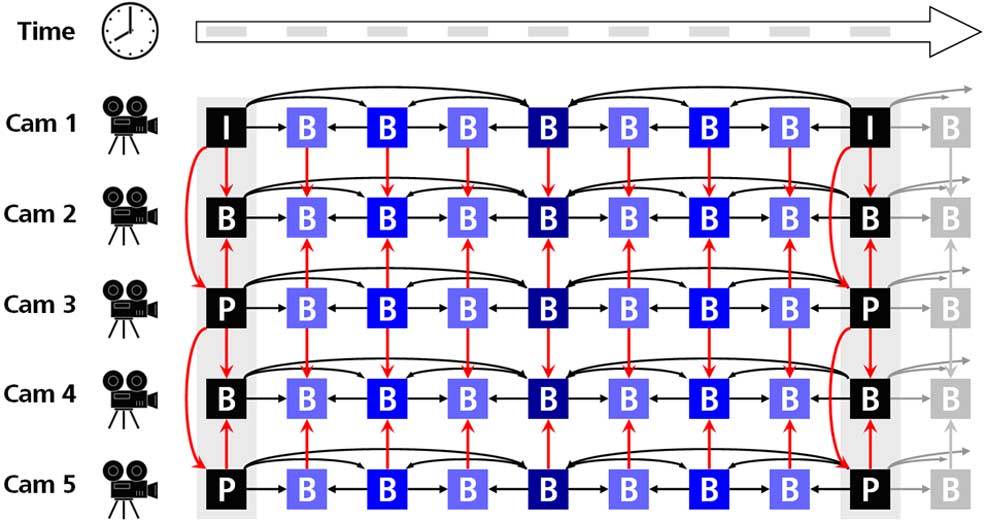
\includegraphics[width=0.8\textwidth]{tempinterpred.jpg}
%\caption{Temporal/inter-view prediction structure for MVC.}
%\label{fig:tempinterpred}
%\end{center}
%\end{figure}
%
%A common element of many 3DTV systems is the use of multiple views of the same scene that have to be transmitted to the user. The straight-forward solution for this would be to encode all video signals independently using a state-of-the-art video codec such as H.264/AVC. However, multiview video contains a large amount of inter-view statistical dependencies, since all cameras capture the same scene from different view-points. These can be exploited for combined temporal/inter-view prediction, as illustrated in Fig. \ref{fig:tempinterpred}. Images are not only predicted from temporally neighbouring images but also from corresponding images in adjacent views. Statistical evaluations have shown that significant gain can be expected from such combined temporal/inter-view prediction \onlinecite{merkle2005statistical, kaup2006analysis}. Pioneering work on multiview image coding is reported in \onlinecite{magnor2000data, magnor2003multi}.
%
%Several research groups addressed multiview video coding (MVC) and developed dedicated inter-view/temporal prediction structures to efficiently exploit all statistical dependencies within the multiview video data sets (see e.g., \onlinecite{oh12542multi, cheng2006multi, yang2006hyper, vetro2004coding, kalva2006design, socek2006permutation, kalva2006challenges, bilen2006multi}. Among those, algorithms that are based on hierarchical B-pictures \onlinecite{schwarz2006analysis} as supported by H.264/AVC syntax in temporal and inter-view dimension (Fig. \ref{fig:tempinterpred}) proved best performance in exhaustive experiments conducted in the context of MPEG standardization \onlinecite{flierl2007motion, merkle2006efficient, mueller2006multi, merkle2007efficient}. In these experiments, it has been shown by objective and subjective measurements that dedicated MVC outperforms independent encoding of the multiple video streams significantly. However, the achievable gain strongly depends on the content and its properties such as camera distance, frame rate and complexity of the content (motion, texture). For some data sets the peak signal-to-noise ratio (PSNR )gain was reported as 0.5 dB and below. Maximum reported gains were up to 3dB.
%
%A drawback of combined temporal/inter-view prediction as illustrated in Fig. \ref{fig:tempinterpred} is the complexity. This includes computational complexity, memory requirements and delay. In \onlinecite{merkle2007efficient, merkle2007coding}, it has been shown that the complexity can be significantly decreased without sacrificing much coding efficiency. Inter-view prediction is restricted here to the key pictures that would be treated as I-pictures in independent encoding of the views (e.g., time and in Fig. \ref{fig:tempinterpred}). Most of the coding gain of MVC comes from inter-view prediction of these pictures that do not use temporal prediction for temporal random access reasons. Omitting inter-view prediction for pictures that have a temporal reference does not cost much coding efficiency whereas it decreases complexity significantly.
%
%In addition to combined temporal/inter-view prediction, specific MVC algorithms have been proposed. The basic idea of depth/disparity-based view interpolation prediction \onlinecite{martinian2006view, kitahara2006multi, martinian2006extensions} is to estimate depth or disparity either at the encoder (this requires overhead for sending the depth/disparity) or the decoder, and to perform view interpolation or 3-D warping for prediction. However, the gains reported so far are marginal. Only for very few test data sets with very close camera settings such view interpolation prediction provides a gain of up to 5\% bit rate saving at the same visual quality. Further investigations are needed to optimize the performance.
%
%Further, illumination and color inconsistencies affect the exploitation of inter-view statistical dependencies. Usually such effects should be minimized by proper setting of the conditions, however, an MVC algorithm should also be able to cope with this as well, since proper white and color balancing of the input can not be guaranteed. Also, the illumination (spotlights, shadows, etc.) varies largely over the multiview images due to the lighting conditions. These problems might be handled by proper illumination and color compensation as proposed in \onlinecite{kim2006results} and \onlinecite{lee2006results}. The basic idea is to modify the motion compensation on macroblock level. Before subtracting the pixel values of the block to be encoded and the reference block, the mean of each is compensated from the corresponding pixel values. This assumes locally constant illumination and color variations, which is an appropriate model trading-off accuracy and complexity. Gains of up to 0.7 dB have been reported for some test data using illumination compensation. However, this strongly depends on the test data and in some cases the gain is negligible or there is none at all. On average over all test data sets a bit rate reduction of 5\% was reported for the same visual quality.
%
%An alternative to illumination compensation on macroblock level integrated into the encoding process, also an appropriate preprocessing can be applied, prior to encoding. Algorithms for illumination correction are well-known in image and video processing. Then the corrected data can be passed to a standard encoder. The big advantage of such an approach is that no changes are necessary to the encoder, decoder and bit stream syntax. A preliminary investigation in this direction is presented in \onlinecite{fecker2006improving}, however, results are not complete and performance in comparison to integrated illumination compensation is not clear.
%
%Another research direction is improving disparity estimation, compensation, and coding \onlinecite{lu2009effective}. Mostly disparity is treated equally to motion, however, it is known that the statistical properties of disparity vectors can be quite different compared to those of motion vectors. Disparity estimation has been studied extensively in the computer vision literature. Usually, basic geometric properties and constraints are taken into account. For instance, the search can be done along epipolar lines.
%
%This may lead to better estimates and reduce the complexity. Further, specific disparity coding may improve the efficiency of inter-view prediction. Specific coding modes for MVC such as the inter-view direct mode \onlinecite{guo2006inter} are under investigation.
%
%Combination of scalability with MVC is investigated for in- stance in \onlinecite{garbas20064d, drose2006extending, yang20064, yang2005scalable, ozbek2006scalable}. So far the feature of scalability only comes with decreased compression efficiency. Distributed MVC is investigated for instance in \onlinecite{guo2006distributed}. Also first work on efficient trans- port and delivery taking user interactivity into account has been presented \onlinecite{kurutepe-interactive, kurutepe2006interactive}. Finally, efficient mechanisms for optimum random access, parallel processing and memory management for MVC have been investigated.
%
%Since the results clearly indicate that MVC outperforms independent encoding of the multiple video signals, and there is a clear demand from industry for a corresponding standard, ISO/ MPEG and ITU/VCEG decided developing a dedicated MVC specification \onlinecite{vetro-joint, vetro2006joint}. It will be an extension of H.264/AVC (Amendment 4), which is scheduled to be finalized in 2008. MVC is the main focus of this Special Issue. We therefore refer the reader to the dedicated articles in this volume that contain all details of state-of-the-art MVC technology.
%
%\subsection{Conclusions and Future Research Directions}
%
%Research on coding of stereo video, multiview video and associated depth or disparity data has reached a good level of maturity. Related international standards are available enabling a variety of 3DTV systems and applications. However, compared to coding of other types of media data the scientific field is relatively young, and therefore there is still a lot of room for improvement of algorithms. This includes for instance optimization of MVC and development of new specific coding MVC algorithms. Depth or disparity coding may be improved further by development of dedicated algorithms. Further, there are more complex types of data representations for 3DTV such as layered depth video and multiview video plus depth that provide extended functionality. Efficient coding algorithms for such data are still under investigation. Initial results are reported in \onlinecite{merkle2007efficientmvc} and \onlinecite{merkle2007multi}. Other types of multiview representations are also under investigation often related to specific types of 3-D displays. An example is presented in \onlinecite{saishu2006flatbed}.
%
%%\cleardoublepage

\chapter{外文资料的书面翻译}

\begin{center}
\heiti{立体电视编解码算法综述}
\end{center}

\section{摘要}

最近,3D电视技术相关的研究工作在全球范围内都有增加。这些研究覆盖了整个媒体处理流程,从采集到显示无所不包。不同的3D电视系统依靠各种类型数据构成的不同的3D场景表示方式。对这些数据的高效编码对于3D电视的成功至关重要。对双目视频、多视点视频、深度图或视差图中像素类型数据的压缩拓展了已有的经典视频编码的原则。针对多视点视频和视频加深度数据的强大算法和开放的国际标准已经出现并一直有着进展,这为在不久的将来引进各种3D电视系统奠定了基础。对3D网格模型的压缩也达到了高度成熟的程度。对静态的几何体,有多种强大的算法可以有效地压缩顶点和连接数据量。对动态3D几何体的压缩是现在更受关注的研究方向。基于时间的预测是一个重要的对动画3D网格序列去冗余信息的机制。容错性对于在易出错的信道上传输数据十分重要,而多描述编码(MDC)是一种可行的保护数据的方法。对静态图和2D视频的MDC已经得到了广泛的研究,但是对多视点视频和3D网格的MDC最近才刚刚提出。用水印进行3D数据的知识产权保护也是一个前沿的研究方向。3D水印方法方面的文献根据表示场景的主要部分在应用算法前后的维数可以归为三类。总而言之,3D电视编码技术正在走向成熟。相关系统和服务可能在不久的将来进入市场。然而,这个方向的研究相对其他媒体数据的研究而言又很少,所以仍有很大的空间可以改进,有很多新的算法可能被提出。

\section{简介}

将我们的视觉延伸到三维空间在近几十年中一直都在研究,但是大规模的消费市场仍然没有发展起来。3D视频还在小众市场发展,包括专业应用(比如科学数据可视化、医药学等)和娱乐方面(比如IMAX影院、3D游戏等)。近年来,更多的研究精力投向了这个领域,以期能够跨越阻碍3D视频应用得到更广泛成功应用的障碍\cite{smolic20063d, onural2004overview, smolic20043dav, smolic2005interactive, onural2006assessment}。从获得信号、处理信号到3D场景表示、编码、传输,再到渲染和3D显示,整个处理流水线的各个部分都取得了显著的进步。很可能在不久的将来,各种3D视频系统、组件、应用和服务就会进入市场。

这一期中给出了各种尖端3D视频技术的综述,分别针对一个3D视频处理流水线中的一个特定组件。这篇文章介绍编码相关的部分。\onlinecite{alatan2007scene}中介绍了用在不同的3D视频系统和应用中的不同3D场景表示格式在。这些格式整合了各种类型的数据,比如多视点视频、深度或3D网格的几何数据。总的来说,3D视频就意味着有大量的数据需要传输、存储和水印。于是高效的压缩就是3D视频成功与否的一个关键条件。同时对发明一个鲁棒的3D水印技术来保护所有权也有很强的需求。此外,开放的国际标准对市场和相关商业的发展也是一个推动力。ISO/IEC JTC1/SC29/WG11 (Moving Picture Experts Group—MPEG)就是一个在数字媒体标准化中起到重要作用的国际标准化组织。所以,这篇文章关注现有的和正在成形的各种数据的MPEG标准。

接下来的几节分别给出多视点视频、深度和关联数据的编码综述,集中关注已有的和正在成形的MPEG标准。第3节介绍用于3D视频表示以及3D计算机图形学的静态和动态3D网格数据的压缩。容错以及3D视频的多描述编码(MDC)在第4节中介绍。然后在第5节中介绍用水印保护3D内容的方法。最后,第6节概况和总结这篇文章的观点。

\section{多视点视频、深度和关联数据编码}

很多3D电视系统都基于场景,这些3D场景由N个相机获取(见\onlinecite{tanimoto2004free, fujii2002free, matsuyama2004real, hamaguchi2003real, carranza2003free, wurmlin20033d, wurmlin20043d, matusik20043d})。最简单的情形就是经典的两路视频构成的立体视频,更复杂一些的系统用8路、16路或更多路相机获取的视频。有些系统还使用可以当作视频信号的深度信息。这一节综述这类数据的压缩算法和标准。更早对这个研究方向的综述可以参见\onlinecite{shum2003survey}。通过共享内容、共享一些相机,多视点视频比起单视点视频的编码可以一定提升。在多视点视频编码中,除了挖掘单个相机的数据在时间上的关联之外,临近的相机之间的关系也被挖掘出来。于是多视点视频在单视点视频的基础上增加了一个新的压缩维度:视点间的方向。

\subsection{传统立体视频编码}

立体视频是多视点视频中最重要的一个特例,是有N=2个视点的情形。 压缩传统的立体视频已经经过了长时间的研究,相关的标准也已经问世。一个传统的立体对由从两个略微不同的视点(对应人的瞳距)观察同一场景的两幅静态图组成。这两幅图片总的来说极其相似,使得它们很适合压缩,比如从一幅图片预测另一幅。例如,其中一幅可以不参考另一幅而单独压缩,而第二幅图片可以从已经编码的一幅图片来预测,就像视频压缩中的基于时间预测的动态补偿那样。
 
对两幅图片的样本基于场景和相机属性(包括位置和相机内部参数比如焦距)的3D几何各自对应起来。每个样本的位移或视差就等价于一个视频序列中两幅连续图像的dense motion field。于是就可以用运动估计和运动补偿一样的方法去做视差分析和视差补偿,以此实现图像预测,然后就只需要编码预测误差或者进一步的残差即可。

然而,一些特定的动态补偿和视差补偿间的区别需要考虑进来。视差向量场的统计与运动向量场的统计不同。视差是有偏的,而且相对较大。零视差以为着一个点在 3D场景中的深度极大,而一个距离相近很近的3D点会有很大的视差值。这需要对视差向量的熵编码做调整。总的来说,在正常的帧率下,视频序列中在时间上邻近的图像倾向于比立体视频的两个视点的图像更加相似。图像损失(内容在一张图中可见但是在另一张图中不存在,也就无法被预测)平均来说在立体视频中出现得比时间上邻近的两幅图更多。此外,立体图片对中的差别可能来自不正确的白平衡或色彩平衡,也可能来自场景的光照和表面反射效果的差别。 

\begin{figure}[htbp]
\begin{center}
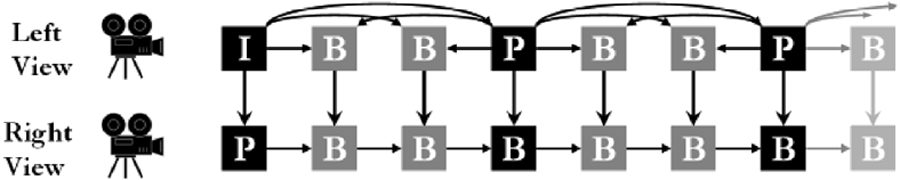
\includegraphics[width=0.8\textwidth]{predh262.png}
\caption{H.262/MPEG-2视频多视点类(multiview profile)的预测示意}
\label{fig:predh262chs}
\end{center}
\end{figure}

视角间和时间上的预测组合是有效压缩传统立体视频的基本方法。对应的标准已经在ITU-T Rec.H.262/ISO/IEC 13818-2 MPEG-2Video, the Multiview Profile\cite{haskell1997digital, itu1994mpeg2}中定义了,如图\ref{fig:predh262chs}所示。左眼视频不参考右眼视频单独编码,使用标准的MPEG-2。这保证了对H.262/MPEG-2的主类(Main Profile)的前向兼容性,因为这样可以解码左眼视频流来显示2D视频。对右眼视频,时间轴预测之外还可以允许做视点间预测。
 
然而,对比分别压缩两个视频流而言,这样的压缩效率提升很有限。这主要是由于基于时间的预测已经达到了很高的性能。特别是当基于时间的预测对于一张特定图像效率不错的时候(比如图\ref{fig:predh262chs}中右眼视频的B帧),那么增加视角间的预测就无法显著提升编码性能了。时间上邻近的图像平均而言一般都比空间上邻近的图像更相似。

对于编码为I帧的图像,也就是说不参考其他视频序列中时间上邻近的帧来编码的帧,加入视角间的预测有明显成效。一般每半秒到一秒时间就会在视频序列中插入这样一个I帧来保证随机访问和容错性。在图\ref{fig:predh262chs}中,左眼序列的最左侧一帧被编码为I帧,当分别编码两个视频序列时,对应的右眼序列中的那一帧也可以编码为I帧。但是在H.262/MPEG-2视频多视点编码中,可以采用视角间预测来达到压缩效率上比编为I帧方式的显著提升。

对于传统立体视频压缩的研究还在各个方向上继续进行着,包括对各个频道的最优码率分配以及放弃前向兼容去设计一个更加有效的视角间预测的结构。相关算法是都是基于更新的视频编码比如H.263\cite{itu1995h263},MPEG-4 Visual\cite{itu1999mpeg4}或H.264/AVC \cite{sun2005stereo, wiegand2003overview, itu2003h264}。但是由于立体视频的应用还没有发展到一个足够大的市场,所有这些进展包括原有的多视点类(Multiview profile)都尚未能商业化。

\subsection{视频加深度数据的压缩}

除了前文描述的经典立体视频外,还有一种传输视频信号的方式——传输一路视频和每个样本的深度图。从视频和深度信息,可以在解码端渲染出一对立体图\cite{fehn2002evolutionary,fehn20043d}。这提供了另一项功能:当用户的头部移动被捕捉到时,能够提供相对应的观察角度的图像。此外,这种格式从压缩效率的角度来看很有价值。深度信息可以被当作单色、仅有明度的视频信号。深度被限制在两个表示对应3D点到摄像机的最小和最大距离的极限距离$Z_{near}$和$Z_{far}$之间。深度范围线性地量子化到8位,也就是最近的点赋值255,最远点赋值为0。这样一来,一张深度图就确定下来了,成为一张灰度图。这些灰阶图可以被插入视频信号的光照信道中,其色彩可以被设定为一个常数。这样获得的标准视频信号就可以用任何先进的视频编码处理了。

欧洲ATTEST的一个项目\cite{fehn2002evolutionary}结果表明深度信息可以用这种方式非常高效地压缩。一些前沿的视频编码参与了测试(MPEG-2, MPEG-4, H.264/AVC)。一项估计显示,只要编码彩色视频信号10\%到20\%的比特率就足以编码高质量的深度信息了。

基于这些观察,这个ATTEST项目提出了一种新的(对比经典的DVB)向前兼容的实现3DTV的方式。它采用一种分层的比特流语法。基层是一个传统的 MPEG-2编码的彩色2D视频。基层可以被任何现有的MPEG-2解码器处理,保证前向兼容性。除此之外,比特流还包含更高一层传输编码后的深度信息。更高级的系统可以访问这一层来解码深度信息,然后通过插值生成一对立体图像来显示。

这种概念由于保证了前向兼容性、压缩率高并且相比传统立体视频功能扩展更多,所以非常有价值。不仅如此,它并不引入一种特定的编码算法。只需要制定一种高层的语法,让解码器能够把输入的两路视频正确地分辨成一路视频和一路深度即可。附加的深度信息($Z_{near}$和$Z_{far}$)需要另外传输。所以MPEG为视频加深度信息制定了一种对应的容器格式 “ISO/IEC 23002-3 Representation of Auxiliary Video and Supplemental Information”,或者称为MPEG-3 Part 3\cite{iso2007rep, iso2007fdam}。此外,H.264/AVC包含一个选项通过辅助的图片语法传输深度图。此处对彩色视频信号和对应的深度视频信号的视频编码都用的是 H.264/AVC。这种方法对任何已部署的H.264/AVC设备都能做到前向兼容。

对视频加深度的格式而言,有一个普遍存在的问题就是深度信息的生成。能够在捕获视频的同时自动获取每个像素深度的摄像机已经问世而且在进一步增强,但是得到的深度场的精度还是很有限。计算机视觉相关的文献中对深度估计的算法有了很深入的研究,强大的解决方案也已经出现。但是这总是一个建立在一定残差误差概率上的估计值。估计的误差会影响渲染出的图像的质量。全自动而且精确的深度获取系统仍然有待开发。对于特定的应用,用户辅助的内容生成可以作为一种选择。即使有了完美的深度图,遮挡也会使渲染出的图像有瑕疵。这些效应在距离原始摄像机位更远的虚拟点上会更加严重。增加一些层(深度视频层作为深度图像层的扩展\cite{shade1998layered})或者扩展到多视点视频加深度\cite{zitnick2004high, kauff2007depth}能够以增加数据量和复杂度为代价,帮助减小这些问题。

\subsection{多视点视频编码}

\begin{figure}[htbp]
\begin{center}
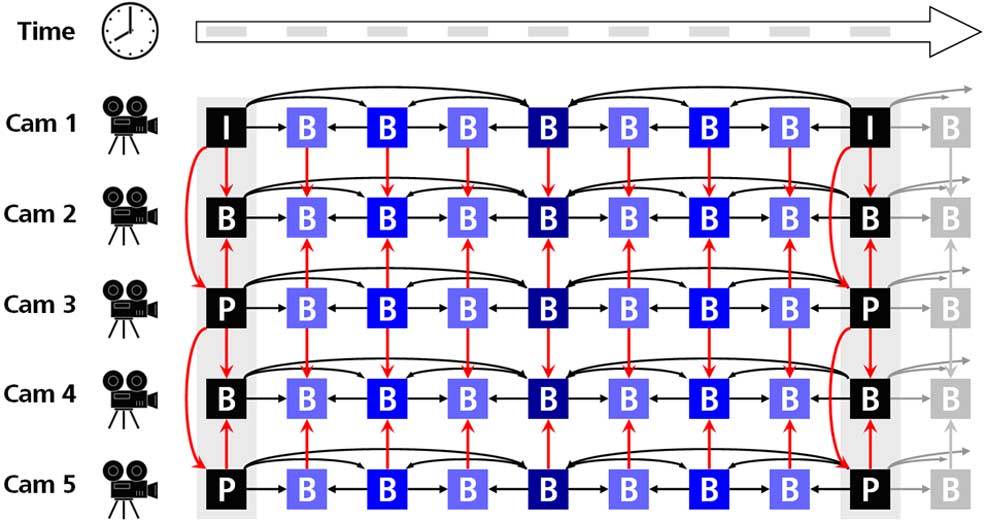
\includegraphics[width=0.8\textwidth]{tempinterpred.jpg}
\caption{MVC的时间和视角间预测结构}
\label{fig:tempinterpredchs}
\end{center}
\end{figure}

3DTV系统的一个共同部分是传输给用户的同一场景不同视角视频的使用。最直接的解决方法就是把所有的视频信号分别用最新的编码方式比如 H.264/AVC编码。但是多视点视频在视角间存在统计意义上很大的相关性,因为每个摄像机捕获的都是不同视角的同一场景的图像。这些相关性可以用来进行时间和视角间预测,如图\ref{fig:tempinterpredchs}所示。图像不仅仅根据时间上临近的图来预测,还根据相邻视角的对应图像预测。统计表明这样的组合式预测能够极大地提高编码效率\cite{merkle2005statistical, kaup2006analysis}。多视点图像编码的前沿研究在\onlinecite{magnor2000data, magnor2003multi}中有报告。

几个研究小组提出了多视点视频(MVC),并且发展了专门的视角间和时间预测的架构来有效地挖掘利用多视点视频数据集中的统计相关性(见\onlinecite{oh12542multi, cheng2006multi, yang2006hyper, vetro2004coding, kalva2006design, socek2006permutation, kalva2006challenges, bilen2006multi})。其中,H.264/AVC时间和视角间预测的语法支持的基于B帧的算法\cite{schwarz2006analysis}在MPEG标准的穷尽测试下被证明是性能最好的\cite{flierl2007motion, merkle2006efficient, mueller2006multi, merkle2007efficient}。在这些实验中,客观和主观的测量都显示MVC极大地超越了独立压缩各个视频。然而,能够获得的提升极其依赖内容和相机间距、帧率、内容复杂度(运动、纹理)等属性。对于一些数据集,信噪比峰值(PSNR)增益在0.5dB以下。最大的增益达到过3dB。

图\ref{fig:tempinterpredchs}中描述的时间和视角间组合预测的一个不足就是其复杂度。包括计算复杂度、内存需求和延迟。在\onlinecite{merkle2007efficient, merkle2007coding}中提到,复杂度在不牺牲多少编码效率的情形下可以极大地降低。视角间预测此时被限制在作为I帧独立编码的关键帧上(例如图\ref{fig:tempinterpredchs}中的$t_0$和$t_8$)。MVC中大部分编码增益来自于这些为了随机访问而不进行视角间预测的帧。忽略有时间预测的帧的视角间预测并不消耗多少编码效率却显著降低复杂度。

在结合时间和视角间预测之外,专门的MVC算法被提了出来。基于深度/视差的视角间插值预测\cite{martinian2006view, kitahara2006multi, martinian2006extensions}的基本思想是在编码(这需要另外传输深度/视差)或解码端估计深度或视差,然后进行视角间插值或者3D扭曲来预测。但是目前得到的增益不高。仅仅对于摄像机参数极其接近的很小一部分数据集,这样的视角间插值预测在同样画质下能节省5\%的比特率。想要优化性能还要做进一步的研究。

不仅如此,光照和色彩的不一致影响了对视角间统计相关性的挖掘。通常这样的效应能被正确的条件设定减小,但是 MVC算法也要能够应对这样的情形,因为输入的白平衡和色彩平衡并不能保证。同样,一定的光照条件下,光照(聚光灯、阴影等)在视角间会有很大的不同。这些问题或许能通过\onlinecite{kim2006results}和\onlinecite{lee2006results}中提出的正确的光照和色彩补偿来解决。基本思想是在宏块级别修改运动补偿。在对待编码帧块和参考块的像素值相减之前,二者的平均值根据对应的像素值做补偿。其中假设了本地的光照和色彩变化是常值,这是个模型的准确率和复杂度之间的权衡。对于一些测试数据,光照补偿获得了0.7dB的增益。但是这个增益极大地依靠测试数据,在一些情况下,增益可以忽略甚至根本不存在。对所有的测试数据集平均下来,相同视觉质量下,能够节省5\%的比特率。

另一种宏块级别的光照补偿可以整合到编码过程中,一个合适的预处理也可以在编码前进行。对图像和视频的光照更正算法广为人知。然后更正过的数据可以被传到一个标准的编码器。这种方法的一大优势是编码器、解码器和码流语法不需要做任何改动。一项这个方向上的前期调研发表在\onlinecite{fecker2006improving}中,但是结果并不完全,性能与整合光照补偿的比较也不清楚。

另一个研究方向是改进视差估计、补偿和编码\cite{lu2009effective}。多数的视差都被当作运动来对待,但是我们知道视差向量的统计属性和运动向量可以完全不同。视差估计在计算机视觉文献中已经被广泛研究。通常,级别的几何属性和约束会考虑进来。比如搜索可以通过沿着核极线(epipolar lines)完成。这可能带来更好的估计和降低复杂度。此外,专门的视差编码或许能提高视角间预测的编码效率。专门的MVC编码模式比如视角间直接模式\cite{guo2006inter}正在研究中。

MVC的扩展性结合正在被研究,比如\onlinecite{garbas20064d, drose2006extending, yang20064, yang2005scalable, ozbek2006scalable}。目前可扩展的功能仅能依靠降低压缩效率。分布式MVC在\onlinecite{guo2006distributed}中被研究。加入用户交互考虑的有效传输在\onlinecite{kurutepe-interactive, kurutepe2006interactive}中初次被讨论。最后,能够随机访问的有效的MVC编码机制、并行处理和内存管理也正在研究中。

由于结果明显表明MVC优于单独编码各路视频信号,业界又显然需要一个对应的标准,ISO/MPEG和ITU/VCEG 决定发展一种专门的MVC标准\cite{vetro-joint, vetro2006joint}。这会是一个H.264/AVC的扩展(第4修正案),这预计在2008年内完工。MVC是这一期特刊的主要关注点。我们因此向读者介绍包含最前沿MVC技术的文章。

\subsection{结论和未来研究方向}

对立体视频、多视点视频和相关深度、视差数据的研究已经有很高的成熟度。相关的国际标准也已经问世,使3DTV系统和应用成为可能。然而,相对于其他类型和媒体数据的编码,这个领域还很年轻,算法还有很大的进步空间。这包括对MVC实力的优化和新的专门的MVC算法的开发。深度和视差编码可能在将来的专门的算法中进一步优化。此外,有更多复杂的3DTV数据结构比如分层的深度视频和多视点视频加深度来提供更多的功能。对这些数据的有效编码算法还在研究之中。初步的结果在\onlinecite{merkle2007efficientmvc}和\onlinecite{merkle2007multi}中有报告。其他多视点描述的类型也在研究中,这往往和特定的一类3D显示器相关。\onlinecite{saishu2006flatbed}中有一个例子。

\begin{center}
\heiti{原文索引}
\end{center}

\noindent \begin{enumerate}
\item[{[1]}] Smolic A, M{\"u}eller K, Stefanoski N, et al. Coding algorithms for 3DTV---a survey. IEEE Transactions on Circuits and Systems for Video Technology, 2007, 17(11):1606-1620
\end{enumerate}

%\cleardoublepage